\documentclass{article}
\usepackage[utf8]{inputenc}
\usepackage[greek,english]{babel}
\usepackage{alphabeta}
\usepackage{fancyhdr}
\usepackage{listings}
\usepackage{mathtools}
\usepackage{siunitx}
\usepackage{xcolor}
\usepackage{graphicx}
\usepackage{pgfplots}
\usepackage[export]{adjustbox}
\usepackage{biblatex}
\addbibresource{ct1-citations.bib}

\title{Εργαστηριακή Εργασία 1 - Εισαγωγή στο Εργαστήριο}
\author{Χρήστος Μαργιώλης - 19390133 \\ Τμήμα 4}
\date{Ιούνιος 2020}

\begin{document}

\begin{figure}[t!]
    \centering
    
\includegraphics[scale=0.3, center]{./res/Logo_University_of_West_Attica.png}
    \Large
    \textbf{Πανεπιστήμιο Δυτικής Αττικής} \\
    \large
    Τμήμα Μηχανικών Πληροφορικής και Ηλεκτρονικών Υπολογιστών \\
    Θεωρία Κυκλωμάτων
\end{figure}
\begin{figure}[b]
    \centering
    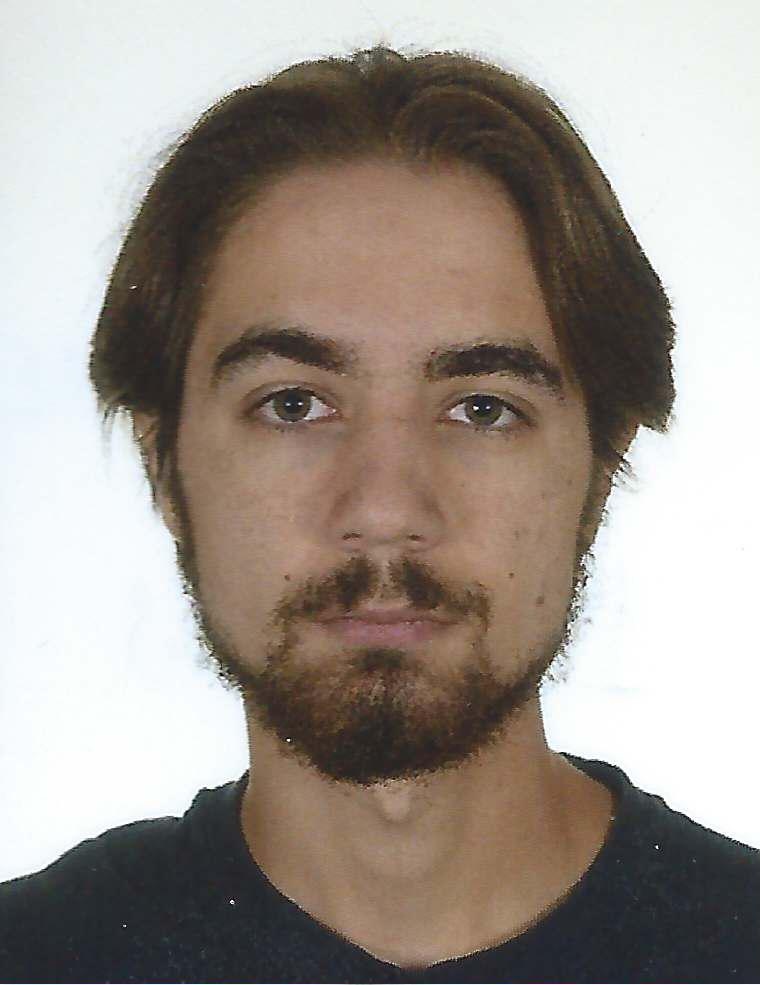
\includegraphics[scale=1]{./res/19390133.jpeg}
\end{figure}

\begin{titlepage}
\maketitle
\end{titlepage}

\renewcommand{\contentsname}{Περιεχόμενα}
\tableofcontents

\renewcommand{\abstractname}{Εισαγωγή}
\begin{abstract}
    Ο σκοπός της εργασίας αυτής είναι η κατανόηση των βασικών εννοιών, νόμων και
    εφαρμογών που υπάρχουν στην επιστήμη της Θεωρίας Κυκλωμάτων.
\end{abstract}
\pagebreak

\section{Συλλογή βιβλιογραφίας}
Η βιβλιογραφία που χρησιμοποιήθηκε, αν και δεν είναι μεγάλη σε έκταση, κάλυψε όλα
τα βασικά προβλήματα της εργασίας. Τα μέρη της βιβλιογραφίας που χρησιμοποιήθηκαν είναι
βασισμένα κυρίως στα θεωρητικά κομμάτια, όπως τις έννοιες και τις μαθηματικές
διατυπώσεις των κανόνων του Kirchhoff, την γραμμικότητα, και τον διαιρέτη τάσης.

\section{Περιγραφή υλοποίησης}
Για την υλοποίηση της εργασίας και βασισμένος στην παραπάνω βιβλιογραφία που συλλέχθηκε,
χρησιμοποίησα μερικά από τα βασικά υλικά ενός κυκλώματος - αντιστάσεις και πηγές.
Εργαλεία που χρησιμοποιήθηκαν είναι το αμπερόμετρο και το βολτόμετρο.

\section{Εργαστηριακό μέρος}
\subsection{Επαλήθευση κανόνων του Kirchhoff}
\subsubsection{Πρώτος κανόνας}
Βάσει του πρώτου κανόνα του Kirchhoff, ισχύει ότι το αλγεβρικό άθροισμα όλων
των ρευμάτων που εισέρχονται ή εξέρχονται σε/από έναν κόμβο είναι ίσο με
μηδέν \cite{papadopoulos}. Αυτό μπορούμε να το εκφράσουμε ως 
\[\sum{I_{in}} = 0\] και \[\sum{I_{out}} = 0\]
Μια εναλλακτική ερμηνεία του πρώτου κανόνα του Kirchhoff είναι ότι το άθροισμα των
ρευμάτων που εισρέουν στον κόμβο είναι ίσο με το άθροισμα των ρευμάτων που εκρέουν
από τον κόμβο, δηλαδή ότι
\[\sum{I_{in}} = \sum{I_{out}}\]
Από την σχέση αυτή είναι ασφαλές να υποθέσουμε, ότι αφού το ρεύμα που θα εισέλθει στον
κόμβο είναι ίσο με το ρεύμα που θα εξέλθει, τότε και το ρεύμα που κυκλοφορεί μέσα στον
κόμβο είναι και αυτό ίσο. \\
Στην προκειμένη περίπτωση, το ρεύμα $I_1$ που εισρέει στον κόμβο σημαίνει ότι είναι
ίσο με τα ρεύματα $I_2$, $I_3$, $I_4$, τα οποία αντιστιχούν στα ρεύματα του κόμβου.
Αντίστοιχα, το ρεύμα $I_5$ που εκρέει από τον κόμβο είναι επίσης ίσο με τα ρεύματα
$I_2$, $I_3$ και $I_4$.

Έτσι, χρησιμοποιώντας τον νόμο του Ohm ώστε να βρούμε τα ρεύματα, έχουμε ότι

\[I_1 = I_2 + I_3 + I_4 = \si{\frac{V_5}{R_{17}} + \frac{V_5}{R_{18}} +
	\frac{V_5}{R_{19}}} = \si{\frac{10\volt}{1\kohm} +
	\frac{10\volt}{1\kohm} + \frac{10\volt}{1\kohm}} =
	\si{30\milli\ampere}\]
Αντίστοιχα
\[I_5 = I_2 + I_3 + I_4 = \si{30\milli\ampere}\]
Άρα καταλήγουμε στο ότι
\[\sum{I_{in}} = 0 \Rightarrow I_1 - I_2 - I_3 - I_4 = 0 \Rightarrow
    \si{(30 - 30)\milli\ampere} = \si{0\milli\ampere}\]
\[\sum{I_{out}} = 0 \Rightarrow I_5 - I_2 - I_3 - I_4 = 0 \Rightarrow
    \si{(30 - 30)\milli\ampere} = \si{0\milli\ampere}\]

Μπορούμε να το επαληθεύσουμε περαιτέρω χρησιμοποιώντας την δεύτερη ερμηνεία του
κανόνα του Kirchhoff. Οπότε έχουμε ότι
\[\sum{I_{in}} = \sum{I_{out}} \Rightarrow I_1 = I_5 \Rightarrow \si{30\milli\ampere} =
        \si{30\milli\ampere} = \si{0\milli\ampere}\]

\subsubsection{Δεύτερος κανόνας}
Ο δεύτερος κανόνας του Kirchhoff μας λέει ότι το αλγεβρικό άθροισμα όλων των τάσεων
κατα μήκος μίας κλειστής διαδρομής ισούται με μηδέν \cite{papadopoulos}.
Με άλλα λόγια μπορούμε να περιγράψουμε το φαινόμενο αυτό ως ότι \textit{το αλγεβρικό
άθροισμα των αυξήσεων τάσεων μείον το άθροισμα των πτώσεων τάσης κατα μήκος μιας
κλειστής διαδρομής είναι ίσο με μηδέν} \cite{mcallister}.
Μπορούμε να εκφράσουμε τις εξής δύο ερμηνείες ως
\[\sum{V_{rise}} - \sum{V_{drop}} = 0 \Rightarrow \sum{V_{rise}} = \sum{V_{drop}}\]
και
\[\sum_{i = loop}{V_{i}} = 0\]
Στην δεύτερη σχέση ουσιαστικά αθροίζουμε όλες τις τάσεις στον βρόχο. \\
Προκειμένου να επαληθεύσουμε τον κανόνα τάσεων του Kirchhoff θα πρέπει
αρχικά να βρούμε την συνολική αντίσταση του κυκλώματος. Εφόσον έχουμε σύνδεση
σε σειρά θα χρειαστούμε τον τύπο
\begin{equation}
	R_T = R_7 + R_8 + R_9
\end{equation}
Αντικαθιστόντας στον τύπο (1) έχουμε
\[R_T = \si{(4,7 + 1 + 1)\kohm} = \si{6,7\kohm}\]
	
Με το παραπάνω αποτέλεσμα θα βρούμε το συνολικό ρεύμα που διαρρέει
στο κύκλωμα χρησιμοποιώντας τον	νόμο του Ohm:
\begin{equation}
	I = \frac{V}{R}
\end{equation}
οπότε έχουμε
\[I = \frac{V_3}{R_T} = \si{\frac{10\volt}{6,7\kohm}} = \si{1,5\milli\ampere}\]

Τώρα, πρέπει να υπολογίσουμε τις εντασεις των ρευμάτων που εισρέουν
και εκρέουν από τον κόμβο.Για να βρούμε τις εντάσεις θα χρησιμοποιήσουμε
τον νόμο του Ohm:
\begin{equation}
	V = I \cdot {R}		
\end{equation}
οπότε έχουμε
\[V_3 =	\si{10\volt}\]
\[V_{M1} = \si{-4,7\kohm \cdot {1,5\milli\ampere}} = \si{-7,0\volt}\]
\[V_{M3} = \si{-1\kohm \cdot {1,5\milli\ampere}} = \si{-1,5\volt}\]
\[V_{M4} = \si{-1\kohm \cdot {1,5\milli\ampere}} = \si{-1,5\volt}\]

Τέλος, αν αθροίσουμε τις παραπάνω έξι εντάσεις, θα επαληθεύσουμε τον
δεύτερο κανόνα του Kirchhoff επειδή προκύπτει οτι το άθροισμα
τους ισούται με μηδέν
\[V_T = V_3 + V_{M1} + V_{M3} + V_{M4} \Rightarrow \]
\[V_T = \si{(10 - 7,0 - 1,5 - 1,5)\volt} = \si{0\volt}\]

\subsection{Γραφική αναπαράσταση σχέσης τάσης-έντασης}
\subsubsection{Σχήμα 3}

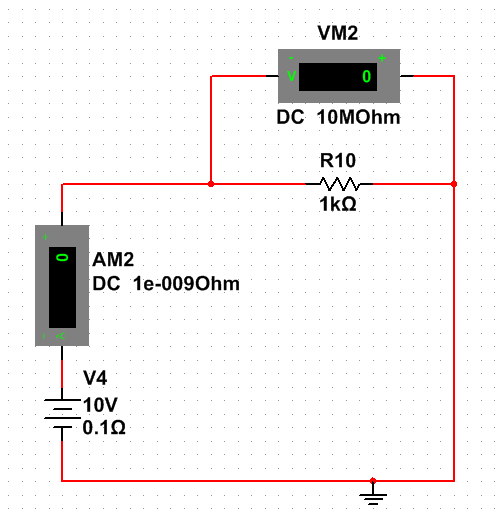
\includegraphics[width=\textwidth]{./res/circ1.png} \\

Από το παραπάνω κύκλωμα προκύπτουν οι ακόλουθες μετρήσεις

\begin{center}
\begin{tabular}{|c|c|c|c|c|c|c|c|c|c|c|c|}
	\hline
	Τάση πηγής (\si{\volt}) & 0 & 1 & 2 & 3 & 4 & 5 & 6 & 7 & 8 & 9 & 10 \\
	\hline
	Ένταση (I)				& 0 & 1 & 2 & 3 & 4 & 5 & 6 & 7 & 8 & 9 & 10 \\
	\hline
	Τάση VM2 (\si{\volt}) & 0 & 1 & 2 & 3 & 4 & 5 & 6 & 7 & 8 & 9 & 10 \\
	\hline
\end{tabular}
\end{center}

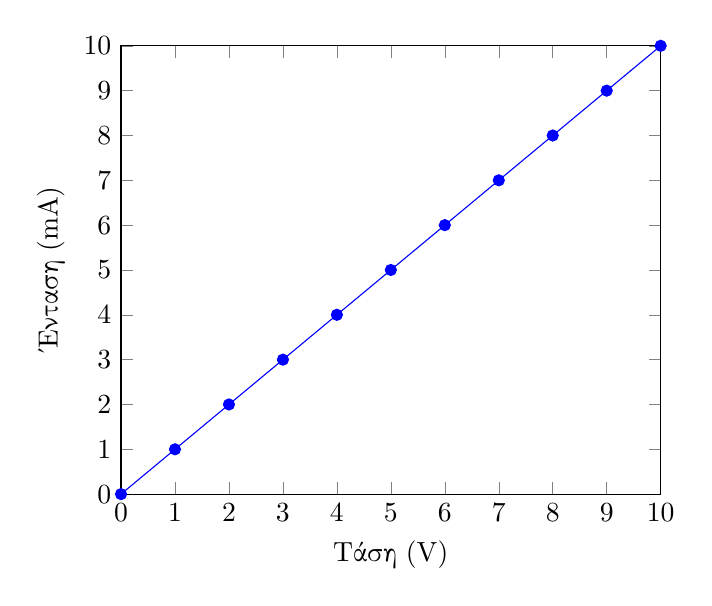
\begin{tikzpicture}
\begin{axis}[
	xlabel={Τάση (\si{\volt})},
	ylabel={Ένταση (\si{\milli\ampere})},
	xmin=0, xmax=10,
	ymin=0, ymax=10,
	xtick={0,1,2,3,4,5,6,7,8,9,10},
	ytick={0,1,2,3,4,5,6,7,8,9,10},
	grid style=dashed,
]
\addplot[
	color=blue,
	mark=*,
]
coordinates {
	(0,0)(1,1)(2,2)(3,3)(4,4)(5,5)(6,6)(7,7)(8,8)(9,9)(10,10)
};
\end{axis}
\end{tikzpicture}

Βάσει του διαγράμματος παρατηρούμε ότι η ένταση του ρεύματος αυξάνεται γραμμικά
όσο αυξάνεται και η τάση. Αυτό συμβαίνει σε γραμμικά κυκλώματα - δηλαδή κυκλώματα
που αποτελούνται από γραμμικά στοιχεία \cite{papadopoulos}. Στην προκειμένη περίπτωση
έχουμε ωμική αντίσταση, η οποία είναι γραμμικό στοιχείο. \\
	
\subsubsection{Σχήμα 4}

\begin{center}
\begin{tabular}{|c|c|c|c|c|c|c|c|c|c|c|}
	\hline
	Αντίσταση (R) \%	& 10 & 20 & 30 & 40 & 50 & 60 & 70 & 80 & 90 & 100 \\
	\hline
	Τάση (\si{\volt})	& 1 & 2 & 3 & 4 & 5 & 6 & 7 &	8 & 9 & 10 \\
	\hline
\end{tabular}
\end{center}

\subsection{Μεταβολή τιμής μεταβλητής αντίστασης}
\subsubsection{Σχήμα 5}

\begin{center}
\begin{tabular}{|c|c|c|c|c|c|c|c|c|c|c|}
	\hline
	Αντίσταση (R) \%	& 10 & 20 & 30 & 40 & 50 & 60 & 70 & 80 & 90 & 100 \\
	\hline
	Ένταση (I) & -1,111 & -1,25 & -1,428 & -1,666 & -2 & -2,5 & -3,333 & -5 & -10 & -75 \\
	\hline
\end{tabular}
\end{center}

\subsection{Ερώτηση 1}
\textit{Τί θα γίνει στο σχήμα 5 αν η μεταβλητή αντίσταση πάει στο 0\%; Υπολογίσατε το
ρεύμα που θα διαρρεύσει την αντίσταση. Υπάρχει τρόπος να επιλυθεί το συγκεκριμένο
πρόβλημα;} \\

Απάντηση: Θα γίνει βραχυκύκλωμα επειδή δεν θα υπάρχει καθόλου αντίσταση. Βραχυκύκλωμα
συμβαίνει γενικότερα όταν υπάρχει ωμική αντίσταση μηδενικής τιμής ή
άπειρης αγωγιμότητας \cite{papadopoulos}. Προκειμένου να λυθεί αυτό το πρόβλημα, πρέπει
να συνδέσουμε άλλη μία αντίσταση ώστε να αποτρέψει το βραχυκύκλωμα σε περίπτωση που η
μεταβλητή αντίσταση πάει στο 0\%.

\subsection{Ερώτηση 2}
\textit{Η μέτρηση της τάσης στο σχήμα 3, θα ήταν ορθότερο να περιλαμβάνει την πτώση
τάσης στα άκρα της αντίστασης και του αμπερομέτρου; Δικαιολογήστε.} \\

Απάντηση: Ναι, θα ήταν ορθότερο η μέτρηση να περιλαμβάνει την πτώση τάσης στα άκρα
της αντίστασης διότι το αμπερόμετρο, παρ'όλο που είναι σχεδιασμένο για όσο μικρότερη
πτώση τάσης, δεν προσφέρει μηδενική πτώση, οπότε αυτό σημαίνει ότι συνδέοντάς το θα
υπάρξει έστω και μικρή πτώση τάσης, και έτσι αν δεν την έχουμε υπολογίσει
είναι πιθανό να μην έχουμε όση ακρίβεια θα θέλαμε στα αποτελέσματά μας.

\subsection{Ερώτηση 3}
\textit{Θεωρήστε διαιρέτη τάσης, όπως στο σχήμα 4, με $R_1 = R_2 = \si{1\kohm}$.
Συνδέουμε φορτίο $R_L = \si{10\ohm}$. Τί θα συμβεί; Προτείνετε τρόπο επίλυσης.} \\

Απάντηση: Συνδέοντας φορτίο $R_L = \si{10\ohm}$ στον διαιρέτη τάσης \cite{harvard}
θα έχουμε πολύ μεγάλη πτώση τάσης. Ένας τρόπος επίλυσης είναι να συνδέσουμε αρκετά
μεγαλύτερο φορτίο $R_L$. Αυτό μπορεί να επιτευχθεί αυξάνοντας την τιμή της αντίστασης
του φορτίου $R_L$.

\renewcommand\refname{Πηγές}
\printbibliography
\end{document}
